%
% A header that lets you compile a chapter by itself, or inside a larger document.
% Adapted from stackoverflow.com/questions/3655454/conditional-import-in-latex
%
%
%Use \inbpdocument and \outbpdocument in your individual files, in place of \begin{document} and \end{document}. In your main file, put in a \def \ismaindoc {} before including or importing anything.
%
% David Duvenaud
% June 2011
% 
% ======================================
%
%


\ifx\ismaindoc\undefined
	\newcommand{\inbpdocument}{
		\def \ismaindoc {}
		% Use this header if we are compiling by ourselves.
		\documentclass[a4paper,11pt,authoryear,index]{common/PhDThesisPSnPDF}
		
%\usepackage{draftwatermark}
%\SetWatermarkLightness{0.95}

% ******************************************************************************
% ****************************** Custom Margin *********************************

% Add `custommargin' in the document class options to use this section
% Set {innerside margin / outerside margin / topmargin / bottom margin}  and
% other page dimensions

\ifsetMargin
\else
    \RequirePackage[left=37mm,right=30mm,top=35mm,bottom=30mm]{geometry}
    \setFancyHdr % To apply fancy header after geometry package is loaded
\fi


%\chead{Unfinished draft}
%\cfoot{\texttt{Unfinished draft - compiled on \today{} at \currenttime}}

% *****************************************************************************
% ******************* Fonts (like different typewriter fonts etc.)*************

% Add `customfont' in the document class option to use this section

\ifsetFont
\else
    % Set your custom font here and use `customfont' in options. Leave empty to
    % load computer modern font (default LaTeX font).  

    \RequirePackage{libertine} 
\fi

% *****************************************************************************
% *************************** Bibliography  and References ********************

%\usepackage{cleveref} %Referencing without need to explicitly state fig /table

% Add `custombib' in the document class option to use this section
\ifsetBib % True, Bibliography option is chosen in class options
\else % If custom bibliography style chosen then load bibstyle here

   \RequirePackage[square, sort, numbers, authoryear]{natbib} % CustomBib

% If you would like to use biblatex for your reference management, as opposed to the default `natbibpackage` pass the option `custombib` in the document class. Comment out the previous line to make sure you don't load the natbib package. Uncomment the following lines and specify the location of references.bib file

% \RequirePackage[backend=biber, style=numeric-comp, citestyle=numeric, sorting=nty, natbib=true]{biblatex}
% \bibliography{References/references} %Location of references.bib only for biblatex

\fi


% changes the default name `Bibliography` -> `References'
\renewcommand{\bibname}{References}


% *****************************************************************************
% *************** Changing the Visual Style of Chapter Headings ***************
% Uncomment the section below. Requires titlesec package.

%\RequirePackage{titlesec}
%\newcommand{\PreContentTitleFormat}{\titleformat{\chapter}[display]{\scshape\Large}
%{\Large\filleft{\chaptertitlename} \Huge\thechapter}
%{1ex}{}
%[\vspace{1ex}\titlerule]}
%\newcommand{\ContentTitleFormat}{\titleformat{\chapter}[display]{\scshape\huge}
%{\Large\filleft{\chaptertitlename} \Huge\thechapter}{1ex}
%{\titlerule\vspace{1ex}\filright}
%[\vspace{1ex}\titlerule]}
%\newcommand{\PostContentTitleFormat}{\PreContentTitleFormat}
%\PreContentTitleFormat


% *****************************************************************************
% **************************** Custom Packages ********************************
% *****************************************************************************


% ************************* Algorithms and Pseudocode **************************

%\usepackage{algpseudocode} 


% ********************Captions and Hyperreferencing / URL **********************

% Captions: This makes captions of figures use a boldfaced small font. 
%\RequirePackage[small,bf]{caption}

\RequirePackage[labelsep=space,tableposition=top]{caption} 
%\renewcommand{\figurename}{Figure} %to support older versions of captions.sty
\captionsetup{labelsep = colon,belowskip=12pt,aboveskip=4pt}

% ************************ Formatting / Footnote *******************************

%\usepackage[perpage]{footmisc} %Range of footnote options 


% ****************************** Line Numbers **********************************

%\RequirePackage{lineno}
%\linenumbers

% ************************** Graphics and figures *****************************

%\usepackage{rotating}
%\usepackage{wrapfig}
%\usepackage{float}
\usepackage{subfig} %note: subfig must be included after the `caption` package. 


% ********************************* Table **************************************

%\usepackage{longtable}
%\usepackage{multicol}
%\usepackage{multirow}
%\usepackage{tabularx}


% ***************************** Math and SI Units ******************************

\usepackage{amsfonts}
\usepackage{amsmath}
\usepackage{amssymb}
%\usepackage{siunitx} % use this package module for SI units


% ******************************************************************************
% ************************* User Defined Commands ******************************
% ******************************************************************************

% *********** To change the name of Table of Contents / LOF and LOT ************

%\renewcommand{\contentsname}{My Table of Contents}
%\renewcommand{\listfigurename}{List of figures}
%\renewcommand{\listtablename}{List of tables}


% ********************** TOC depth and numbering depth *************************

\setcounter{secnumdepth}{2}
\setcounter{tocdepth}{2}

% ******************************* Nomenclature *********************************

% To change the name of the Nomenclature section, uncomment the following line

%\renewcommand{\nomname}{Symbols}


% ********************************* Appendix ***********************************

% The default value of both \appendixtocname and \appendixpagename is `Appendices'. These names can all be changed via: 

%\renewcommand{\appendixtocname}{List of appendices}
%\renewcommand{\appendixname}{Appndx}

		% All my custom preamble stuff.  Shouldn't overlap with anything in official-preamble




% Paths to figure and table directories.
\newcommand{\symmetryfigsdir}{figures/symmetries}
\newcommand{\topologyfiguresdir}{figures/topology}
\newcommand{\infinitefiguresdir}{figures/infinite}
\newcommand{\grammarfiguresdir}{figures/grammar}
\newcommand{\introfigsdir}{figures/intro}
\newcommand{\gplvmfiguresdir}{figures/gplvm}
\newcommand{\warpedfiguresdir}{figures/warped-mixtures}
\newcommand{\deeplimitsfiguresdir}{figures/deep-limits}
\newcommand{\quadraturefigsdir}{figures/quadrature}
\newcommand{\additivefigsdir}{figures/additive}
\newcommand{\decompfigsdir}{figures/decomp}
\newcommand{\examplefigsdir}{figures/worked-example}

\usepackage{bm}  % for warped mixtures - is this necessary?
\usepackage{booktabs}
\usepackage{tabularx}
\usepackage{multirow}
\usepackage{datetime}
\renewcommand{\tabularxcolumn}[1]{>{\arraybackslash}m{#1}}
\usepackage{relsize}
\usepackage{graphicx}
\usepackage{amsmath,amssymb,textcomp}
\usepackage{nicefrac}
\usepackage{amsthm}
\usepackage{tikz}
\usetikzlibrary{arrows}
\usetikzlibrary{calc}
\usepackage{nth}
\usepackage{rotating}
\usepackage{array}
\usepackage{fp}
\usepackage{cleveref}   % Note: this package sometimes causes the page counter to reset.
\crefname{equation}{equation}{equations}
\crefname{figure}{figure}{figures}
%\usepackage{common/sectsty}

% Controls capitalization of all headers
%\usepackage{stringstrings}
%\usepackage[explicit]{titlesec}
%\newcommand\SentenceCase[1]{%
%  \caselower[e]{#1}%
%  \capitalize[q]{\thestring}%
%}
%\titleformat{\section}
%  {\normalfont\Large\bfseries}{\thesection}{1em}{\SentenceCase{#1}\thestring}


%\titleformat{\section} % The normal, unstarred version
%    {\Large\bfseries}{}{2ex}
%    {\thesection. \MakeSentenceCase{#1}}

%\titleformat{name=\section,numberless} % The starred version; note the `numberless` key
%    {\Large\bfseries}{}{2ex}
%    {\MakeSentenceCase{#1}}

\usepackage[hyperpageref]{backref}
% Setup to show (pages 4 and 9) sort of thing in the bibliography - DD
%\def\foo{\hspace{\fill}\mbox{}\linebreak[0]\hspace*{\fill}}
%\def\foo{\parbox{3cm}{\hfill}
%\def\foo{\parbox{3cm}{\hfill}
%\newcommand\foo[1]{{\raggedleft{\hfill{\mbox{\hfill{#1}}}}}}
\newcommand{\comfyfill}[1]{% = Thorsten Donig's \signed
  \unskip\hspace*{0.1em plus 1fill}
  \nolinebreak[3]%
  \hspace*{\fill}\mbox{#1}
  \parfillskip0pt\par
}
\newcommand\foo[1]{{\comfyfill{\mbox{#1}}}}
%\newcommand\foo[1]{{\mbox{#1}}}
\renewcommand*{\backref}[1]{}
\renewcommand*{\backrefalt}[4]{%
\ifcase #1 %
%
\or
\foo{(page #2)}%
\else
\foo{(pages #2)}%
\fi
}

\usepackage{stringstrings}

%\newcommand{\headercase}{\
%\DeclareFieldFormat{titlecase}{\MakeSentenceCase{#1}}


%% For submission, make all render blank.
%%%%%%%%%%%%%%%%%%%%%%%%%%%%%%%%%%%%%%%%%%%%%%%%%%%%%%%%%%
%%%% EDITING HELPER FUNCTIONS  %%%%%%%%%%%%%%%%%%%%%%%%%%%
%%%%%%%%%%%%%%%%%%%%%%%%%%%%%%%%%%%%%%%%%%%%%%%%%%%%%%%%%%

%% NA: needs attention (rough writing whose correctness needs to be verified)
%% TBD: instructions for how to fix a gap ("Describe the propagation by ...")
%% PROBLEM: bug or missing crucial bit 

%% use \fXXX versions of these macros to put additional explanation into a footnote.  
%% The idea is that we don't want to interrupt the flow of the paper or make it 
%% impossible to read because there are a bunch of comments.

%% NA's (and TBDs, those less crucially) should be written so 
%% that they flow with the text.

\definecolor{WowColor}{rgb}{.75,0,.75}
\definecolor{SubtleColor}{rgb}{0,0,.50}

% inline
\newcommand{\NA}[1]{\textcolor{SubtleColor}{ {\tiny \bf ($\star$)} #1}}
\newcommand{\LATER}[1]{\textcolor{SubtleColor}{ {\tiny \bf ($\dagger$)} #1}}
\newcommand{\TBD}[1]{\textcolor{SubtleColor}{ {\tiny \bf (!)} #1}}
\newcommand{\PROBLEM}[1]{\textcolor{WowColor}{ {\bf (!!)} {\bf #1}}}

% as margin notes

\newcounter{margincounter}
\newcommand{\displaycounter}{{\arabic{margincounter}}}
\newcommand{\incdisplaycounter}{{\stepcounter{margincounter}\arabic{margincounter}}}

\newcommand{\fTBD}[1]{\textcolor{SubtleColor}{$\,^{(\incdisplaycounter)}$}\marginpar{\tiny\textcolor{SubtleColor}{ {\tiny $(\displaycounter)$} #1}}}

\newcommand{\fPROBLEM}[1]{\textcolor{WowColor}{$\,^{((\incdisplaycounter))}$}\marginpar{\tiny\textcolor{WowColor}{ {\bf $\mathbf{((\displaycounter))}$} {\bf #1}}}}

\newcommand{\fLATER}[1]{\textcolor{SubtleColor}{$\,^{(\incdisplaycounter\dagger)}$}\marginpar{\tiny\textcolor{SubtleColor}{ {\tiny $(\displaycounter\dagger)$} #1}}}

%\renewcommand{\LATER}[1]{}
%\renewcommand{\fLATER}[1]{}
%\renewcommand{\TBD}[1]{}
%\renewcommand{\fTBD}[1]{}
%\renewcommand{\PROBLEM}[1]{}
%\renewcommand{\fPROBLEM}[1]{}
%\renewcommand{\NA}[1]{}


% HUMBLE WORDS: shown slightly smaller when in normal text
% Thanks to Christian Steinruecken!

% HUMBLE WORDS: shown slightly smaller when in normal text
% Christian Steinruecken
%
\makeatletter%
%\def\@humbleformat#1{{\fontsize{}{1em}\selectfont #1}}
%\def\@humbleformat#1{\textsmaller{#1}}%
\newlength{\nonHumbleHeight}
\def\@humbleformat#1{{\settoheight{\nonHumbleHeight}{#1}\resizebox{!}{0.94\nonHumbleHeight}{#1}}}%
\def\@idxhumbleformat#1{{\relscale{0.95}{#1}}}%
%\def\@humbleformat#1{{#1}}%
\def\declareHumble#1#2{%
  \expandafter\def\csname #1\endcsname{\@humbleformat{#2}}%
  \expandafter\def\csname s#1\endcsname{{#2}}%
  \expandafter\def\csname idx#1\endcsname{{\@idxhumbleformat{#2}}}%
}%
\def\humble#1{\@humbleformat{#1}}%
\def\idxhumble#1{\@idxhumbleformat{#1}}%
\makeatother%

% Convenient indexing for humble abbreviations
\def\humbleindex#1#2{\index{#1@\idxhumble{#1}}}



% TODO: Clean up duplicates
\declareHumble{ANOVA}{ANOVA}
\declareHumble{ARD}{ARD}
\declareHumble{BIC}{BIC}
\declareHumble{BMC}{BMC}
\declareHumble{bq}{BQ}
\declareHumble{CRP}{CRP}
\declareHumble{dirpro}{DP}
\declareHumble{HDMR}{HDMR}
\declareHumble{GAM}{GAM}
\declareHumble{GEM}{GEM}
\declareHumble{GMM}{GMM}
\declareHumble{gplvm}{GP-LVM}
\declareHumble{gpml}{GPML}
\declareHumble{GPML}{GPML}
\declareHumble{gprn}{GPRN}
\declareHumble{gpt}{GP}
\declareHumble{gp}{GP}
\declareHumble{HKL}{HKL}
\declareHumble{HMC}{HMC}
\declareHumble{ibp}{IBP}
\declareHumble{iGMM}{iGMM}
\declareHumble{iwmm}{iWMM}
\declareHumble{kCP}{CP}
\declareHumble{kCW}{CW}
\declareHumble{kC}{C}
\declareHumble{KDE}{KDE}
\declareHumble{kLin}{Lin}
\declareHumble{KPCA}{KPCA}
\declareHumble{kPer}{Per}
\declareHumble{kPerGen}{ZMPer}
\declareHumble{kRQ}{RQ}
\declareHumble{kSE}{SE}
\declareHumble{kWN}{WN}
\declareHumble{Lin}{Lin}
\declareHumble{LBFGS}{L-BFGS}
\declareHumble{LIBSVM}{LIBSVM}
\declareHumble{MAP}{MAP}
\declareHumble{mcmc}{MCMC}
\declareHumble{MKL}{MKL}
\declareHumble{MLP}{MLP}
\declareHumble{MNIST}{MNIST}
\declareHumble{MSE}{MSE}
\declareHumble{OU}{OU}
\declareHumble{Per}{Per}
\declareHumble{RBF}{RBF}
\declareHumble{RMSE}{RMSE}
\declareHumble{RQ}{RQ}
\declareHumble{SBQ}{SBQ}
\declareHumble{seard}{SE-ARD}
\declareHumble{sefull}{SE-\textnormal{full}}
\declareHumble{SEGP}{SE-GP}
\declareHumble{SE}{SE}
\declareHumble{SNR}{SNR}
\declareHumble{SSANOVA}{SS-ANOVA}
\declareHumble{SVM}{SVM}
\declareHumble{UCI}{UCI}
\declareHumble{UMIST}{UMIST}
\declareHumble{vbgplvm}{VB GP-LVM}

\newcommand{\kSig}{\boldsymbol\sigma}

\def\subexpr{{\cal S}}
\def\baseker{{\cal B}}
\def\numWinners{k}

\def\ie{i.e.\ }
\def\eg{e.g.\ }
\def\etc{etc.\ }
\let\oldemptyset\emptyset
%\let\emptyset 0




% Unify notation between neural-net land and GP-land.
\newcommand{\hphi}{h}
\newcommand{\hPhi}{\vh}
\newcommand{\walpha}{w}
\newcommand{\wboldalpha}{\bw}
\newcommand{\wcapalpha}{\vW}
\newcommand{\lengthscale}{w}

\newcommand{\layerindex}{\ell}



\newcommand{\gpdrawbox}[1]{
\setlength\fboxsep{0pt}
\hspace{-0.15in} 
\fbox{
\includegraphics[width=0.464\columnwidth]{\deeplimitsfiguresdir/deep_draws/deep_gp_sample_layer_#1}
}}



\newcommand{\procedurename}{ABCD}
\newcommand{\genText}[1]{{\sf #1}}



\newcommand{\asdf}{$^{\textnormal{th}}$}

\newcommand{\binarysum}{\sum_{\bf{x} \in \{0,1\}^D}}
\newcommand{\expect}{\mathbb{E}}
\newcommand{\expectargs}[2]{\mathbb{E}_{#1} \left[ {#2} \right]}
\newcommand{\var}{\mathbb{V}}
\newcommand{\varianceargs}[2]{\mathbb{V}_{#1} \left[ {#2} \right]}
\newcommand{\cov}{\operatorname{cov}}
\newcommand{\Cov}{\operatorname{Cov}}
\newcommand{\covargs}[2]{\Cov \left[ {#1}, {#2} \right]}
\newcommand{\variance}{\mathbb{V}}
\newcommand{\vecop}[1]{\operatorname{vec} \left( {#1} \right)}

\newcommand{\covarianceargs}[2]{\Cov_{#1} \left[ {#2} \right]}
\newcommand{\colvec}[2]{\left[ \begin{array}{c} {#1} \\ {#2} \end{array} \right]}
\newcommand{\tbtmat}[4]{\left[ \begin{array}{cc} {#1} & {#2} \\ {#3} & {#4} \end{array} \right]}

\newcommand{\acro}[1]{{\humble{#1}}}
%\newcommand{\vect}[1]{\boldsymbol{#1}}
\newcommand{\vect}[1]{{\bf{#1}}}
\newcommand{\mat}[1]{\mathbf{#1}}
\newcommand{\pderiv}[2]{\frac{\partial #1}{\partial #2}}
\newcommand{\npderiv}[2]{\nicefrac{\partial #1}{\partial #2}}

\newcommand{\pha}{^{\phantom{:}}}

\newcommand{\argmin}{\operatornamewithlimits{argmin}}
\newcommand{\argmax}{\operatornamewithlimits{argmax}}

% The following designed for probabilities with long arguments

\newcommand{\Prob}[2]{P\!\left(\,#1\;\middle\vert\;#2\,\right)}
\newcommand{\ProbF}[3]{P\!\left(\,#1\!=\!#2\;\middle\vert\;#3\,\right)}
\newcommand{\p}[2]{p\!\left(#1\middle\vert#2\right)}
\newcommand{\po}[1]{p\!\left(#1\right)}
\newcommand{\pF}[3]{p\!\left(\,#1\!=\!#2\;\middle\vert\;#3\,\right)} 
\newcommand{\mean}[2]{{m}\!\left(#1\middle\vert#2\right)}



\newcommand{\valpha}{\boldsymbol{\alpha}}
\newcommand{\va}{\vect{a}}
\newcommand{\vA}{\vect{A}}
\newcommand{\vB}{\mat{B}}
\newcommand{\vb}{\vect{b}}
\newcommand{\vC}{\mat{C}}
\newcommand{\vc}{\vect{c}}
\newcommand{\vecf}{\boldsymbol{f}}
\newcommand{\vell}{\vect{\ell}}
\newcommand{\vepsilon}{\boldsymbol{\epsilon}}
\newcommand{\veps}{\boldsymbol{\epsilon}}
\newcommand{\ve}{\boldsymbol{\epsilon}}
\newcommand{\vf}{\vecf}
\newcommand{\vg}{\vect{g}}
\newcommand{\vh}{\vect{h}}
\newcommand{\vI}{\mat{I}}
\newcommand{\vK}{\mat{K}}
\newcommand{\vk}{\vect{k}}
\newcommand{\vL}{\mat{L}}
\newcommand{\vl}{\vect{l}}
\newcommand{\vmu}{{\boldsymbol{\mu}}}
\newcommand{\vone}{\vect{1}}
\newcommand{\vphi}{{\boldsymbol{\phi}}}
\newcommand{\vpi}{{\boldsymbol{\pi}}}
\newcommand{\vq}{\vect{q}}
\newcommand{\vR}{\mat{R}}
\newcommand{\vr}{\vect{r}}
\newcommand{\vsigma}{{\boldsymbol{\sigma}}}
\newcommand{\vSigma}{\mat{\Sigma}}
\newcommand{\vS}{\mat{S}}
\newcommand{\vs}{\vect{s}}
\newcommand{\vtheta}{{\boldsymbol{\theta}}}
\newcommand{\vu}{\vect{u}}
\newcommand{\vV}{\mat{V}}
\newcommand{\vW}{\mat{W}}
\newcommand{\vw}{\vect{w}}
\newcommand{\vX}{\mat{X}}
\newcommand{\vx}{\vect{x}}
\newcommand{\vY}{\mat{Y}}
\newcommand{\vy}{\vect{y}}
\newcommand{\vzero}{\vect{0}}
\newcommand{\vZ}{\mat{Z}}
\newcommand{\vz}{\vect{z}}


% deep gp notation
\newcommand{\netweights}{w}
\newcommand{\vnetweights}{\vw}
\newcommand{\mnetweights}{\vW}
\newcommand{\outweights}{\v}
\newcommand{\voutweights}{\vv}
\newcommand{\moutweights}{\vV}

\newcommand{\unitparams}{\v}
\newcommand{\vunitparams}{\vv}
\newcommand{\munitparams}{\vV}


\newcommand{\He}{\mathcal{H}}
\newcommand{\normx}[2]{\left\|#1\right\|_{#2}}
\newcommand{\Hnorm}[1]{\normx{#1}{\He}}
\newcommand{\mmd}{{\rm MMD}}


\newcommand{\mf}{\bar{\vf}}

%\newcommand{\mf}{\mu} %{\bar{\ell}}
\newcommand{\lf}{f} % Likelihood function
\newcommand{\st}{_\star}

% from simpler log-bq writeup
\newcommand{\lftwo}{{\log \ell}}
\newcommand{\mftwo}{{\bar \ell}}
\newcommand{\loggp}{{\log\acro{GP}}}%| \bX, \vy )}}
\newcommand{\loggpdist}{{\acro{GP}(\lftwo)}}%| \vX, \vy )}}


\newcommand{\inv}{^{{\mathsmaller{-1}}}}
\newcommand{\tohalf}{^{{\mathsmaller{\nicefrac{1}{2}}}}}

\newcommand{\Normal}{\mathcal{N}}
\newcommand{\N}[3]{\mathcal{N}\!\left(#1 \middle| #2,#3\right)}
\newcommand{\Nt}[2]{\mathcal{N}\!\left(#1,#2\right)}
\newcommand{\NT}[2]{\mathcal{N}\!\left(#1,#2\right)}
\newcommand{\GPdist}[3]{\mathcal{GP}\!\left(#1 \, \middle| \, #2, #3 \right)}
\newcommand{\GPdisttwo}[2]{\mathcal{GP}\!\left(\, #1, #2 \right)}
\newcommand{\bN}[3]{\mathcal{N}\big(#1 \middle| #2,#3\big)}
\newcommand{\boldN}[3]{\text{\textbf{\mathcal{N}}}\big(#1;#2,#3\big)}
\newcommand{\ones}[1]{\mat{1}_{#1}}
\newcommand{\eye}[1]{\mat{E}_{#1}}
\newcommand{\tra}{^{\mathsf{T}}}
%\newcommand{\tra}{^{\top}}
%\mathsf{T}
\newcommand{\trace}{\operatorname{tr}}
\newcommand{\shift}{\operatorname{shift}}
\renewcommand{\mod}{\operatorname{mod}}
\newcommand{\deq}{:=}
\newcommand{\oneofk}{\operatorname{one-of-k}}
%\newcommand{\degree}{^\circ}

\newcommand{\GPt}[2]{\mathcal{GP}\!\left(#1,#2\right)}
%\newcommand{\GPt}[2]{\gp\!\left(#1,#2\right)}

\DeclareMathOperator{\tr}{tr}
\DeclareMathOperator{\chol}{chol}
\DeclareMathOperator{\diag}{diag}

\newenvironment{narrow}[2]{%
  \begin{list}{}{%
  \setlength{\topsep}{0pt}%
  \setlength{\leftmargin}{#1}%
  \setlength{\rightmargin}{#2}%
  \setlength{\listparindent}{\parindent}%
  \setlength{\itemindent}{\parindent}%
  \setlength{\parsep}{\parskip}}%
\item[]}{\end{list}}



\newcommand{\dist}{\ \sim\ }
\def\given{\,|\,}

% Table stuff
\newcolumntype{C}[1]{>{\centering\let\newline\\\arraybackslash\hspace{0pt}}m{#1}}
\newcolumntype{L}[1]{>{\raggedright\let\newline\\\arraybackslash\hspace{0pt}}m{#1}}
\newcolumntype{R}[1]{>{\raggedleft\let\newline\\\arraybackslash\hspace{0pt}}m{#1}}

\newcommand{\defeq}{\mathrel{:\mkern-0.25mu=}}

\def\ie{i.e.\ }
\def\eg{e.g.\ }
\def\iid{i.i.d.\ }
%\def\simiid{\sim_{\mbox{\tiny iid}}}
\def\simiid{\overset{\mbox{\tiny iid}}{\sim}}
\def\simind{\overset{\mbox{\tiny \textnormal{ind}}}{\sim}}
\def\eqdist{\stackrel{\mbox{\tiny d}}{=}}
%\newcommand{\distas}[1]{\mathbin{\overset{#1}{\kern \z@ \sim}}}
%TODO: fix this - it worked outside the thesis!
\newcommand{\distas}[1]{\mathbin{\overset{#1}{\sim}}}

\def\Reals{\mathbb{R}}

\def\Uniform{\mbox{\rm Uniform}}
\def\Bernoulli{\mbox{\rm Bernoulli}}
\def\GP{\mathcal{GP}}
\def\GPLVM{\mathcal{GP-LVM}}




% Kernel stuff

\def\iva{\vect{\inputVar}}
\def\ivaone{\inputVar}
\def\inputVar{x}
\def\InputVar{X}
\def\InputSpace{\mathcal{X}}
\def\outputVar{y}
\def\OutputSpace{\mathcal{Y}}
\def\function{f}
\def\kernel{k}
\def\KernelMatrix{K}
\def\SumKernel{\sum}
\def\ProductKernel{\prod}
\def\expression{e}
\def\feat{\vh}

\newcommand{\kerntimes}{ \! \times \!}
\newcommand{\kernplus}{ \, + \,}


% Proof stuff
\theoremstyle{plain}
\newtheorem{theorem}{Theorem}[section]
\newtheorem{lemma}[theorem]{Lemma}
\newtheorem{prop}[theorem]{Proposition}
\newtheorem{proposition}{Proposition}
\newtheorem*{cor}{Corollary}

% For infinite bq
\newcommand{\iv}{\theta}
\newcommand{\viv}{\vtheta}

% For intro chapter
\newcommand{\funcval}{\vf(\vX)}
\newcommand{\testpoint}{{\vx^\star}}

\newcommand{\underwrite}[2]{{\underbrace{#1}_{\textnormal{#2}}}}



% For kernel figures
\newcommand{\fhbig}{2cm}%
\newcommand{\fwbig}{3cm}%
\newcommand{\kernpic}[1]{\includegraphics[height=\fhbig,width=\fwbig]{\grammarfiguresdir/structure_examples/#1}}%
\newcommand{\kernpicr}[1]{\rotatebox{90}{\includegraphics[height=\fwbig,width=\fhbig]{\grammarfiguresdir/structure_examples/#1}}}%
\newcommand{\addkernpic}[1]{{\includegraphics[height=\fhbig,width=\fwbig]{\grammarfiguresdir/additive_multi_d/#1}}}%
\newcommand{\largeplus}{\tabbox{{\Large+}}}%
\newcommand{\largeeq}{\tabbox{{\Large=}}}%
\newcommand{\largetimes}{\tabbox{{\Large$\times$}}}%
\newcommand{\fixedx}{$x$ (with $x' = 1$)}%

% for warped mixtures
\newcommand{\CLAS}{\vz}  %cluster assignments
\newcommand{\CLASi}{z} % individual cluster assignments


		% ************************ Thesis Information & Meta-data **********************

%% The title of the thesis
\title{Automating statistical modelling}

%\texorpdfstring is used for PDF metadata. Usage:
%\texorpdfstring{LaTeX_Version}{PDF Version (non-latex)} eg.,
%\texorpdfstring{$sigma$}{sigma}

%% The full name of the author
\author{James Robert Lloyd}

%% Department (eg. Department of Engineering, Maths, Physics)
%\dept{Department of Engineering}

%% University and Crest
\university{University of Cambridge}
\crest{
\includegraphics[width=0.25\textwidth]{misc/University_Crest}}

%% You can redefine the submission text:
% Default as per the University guidelines: This dissertation is submitted for
% the degree of Doctor of Philosophy
%\renewcommand{\submissiontext}{change the default text here if needed}

%% Full title of the Degree 
\degree{Doctor of Philosophy}
 
%% College affiliation (optional)
\college{Trinity College}

%% Submission date
\degreedate{December 2014} 

%% Meta information
\subject{Machine Learning}
\keywords{{LaTeX} {PhD Thesis} {Engineering} {University of Cambridge} {Machine Learning} {Gaussian processes} {Time Series} {Model checking} {Model criticism} {Aldous--Hoover} {Networks}}



		\begin{document}
	}	
	\newcommand{\outbpdocument}[1]{
		% Fake chapters so references aren't broken
		\label{ch:intro}                
		\label{ch:dummy}
		\label{ch:discussion}
		%\bibliographystyle{common/CUEDthesis}
		\bibliographystyle{plainnat}
		\bibliography{references.bib}
		\end{document}
	}	
\else
	%If we're inside another document, no need to re-start the document.
	\ifx\inbpdocument\undefined
		\newcommand{\inbpdocument}{}
		\newcommand{\outbpdocument}[1]{}
	\fi
\fi

\inbpdocument

\chapter{Statistical models for networks}
\label{ch:networks}

This chapter\dots

\section{Introduction}


Relational data records relations between entities in a given set. Such data
arises in a variety of contexts, including graph-valued data 
\citep[e.g.][]{Airoldi2008,Hoff2002}, micro-array data, tensor data 
\citep[e.g.][]{Xu:Yan:Qi:2012} and collaborative filtering
\citep[e.g.][]{Salakhutdinov2008}.
Pairwise relations can be summarized in a 2-dimensional array (a matrix);
more generally, relations between $d$-tuples are recorded as $d$-dimensional arrays.
We consider Bayesian models of infinite 2-arrays $(\darray_{ij})_{i,j\in\Nats}$, where entries $\darray_{ij}$ take values in a space $\dataspace$. 
Each entry $\darray_{ij}$ describes the relation between objects $i$ and $j$. Finite
samples---relational measurements for $n$ objects---are $n\times n$-arrays. As the sample size increases, the data aggregates into
a larger and larger array. 
Graph-valued data, for example, corresponds to the case $\dataspace=\lbrace{0,1}\rbrace$.
In collaborative filtering problems, the set of objects
is subdivided into two disjoint sets, \eg users and items. This corresponds to a bipartite graph if the relations are additionally binary.

Latent variable models for relational data explain observations by means of an underlying structure
or summary,
such as a low-rank approximation to an observed matrix or an embedding into a Euclidean space.
This structure is formalized as an latent (unobserved) variable.
Examples of such models include probabilistic matrix factorization (PMF) \citep{Salakhutdinov2008}, the eigenmodel of 
\citet{Hoff2007a}, the mixed-membership stochastic blockmodel (MMSB) \citep{Airoldi2008}
and the Gaussian process latent variable model (GPLVM) \citep[e.g.][]{Lawrence2009}.

\citet{Hoff2007a} first noted that latent variable models can be justified by an exchangeability argument.
Building on this connection, we consider nonparametric models for graphs and arrays.
Results of
Aldous \cite{Aldous:1981}, Hoover \cite{Hoover:1979} and Kallenberg \cite{Kallenberg:1992} show
that random arrays which satisfy an exchangeability property can be represented in terms of a random
function. These representations have been further developed in discrete analysis for the
special case of graphs \citep{Lovasz:Szegedy:2006}; this case is illustrated in Fig.~\ref{fig:W:graph}.
The results can be regarded as a generalization of de Finetti's theorem to array-valued data.
Their implication for Bayesian modeling is that
\emph{we can specify a prior for an exchangeable random array model by specifying a prior on (measurable) functions}.
The prior is in general a distribution on the space of all functions which can arise in the representation
result, and the dimension of this space is infinite. A prior must hence be nonparametric to have reasonably large support;
a parametric prior concentrates on a finite-dimensional subset.
In the following, we model the representing function explicitly using a nonparametric prior.

\begin{figure}
 \begin{center}
    \begin{tikzpicture}[>=stealth,scale=2.4]%,transform canvas={xshift=-3cm,yshift=1cm}]
  \begin{scope}[yshift=0.5cm]
  \begin{scope}
    %\path[use as bounding box] (-0.5,0.5) rectangle (2.8,-1.5);
    \draw (0,0) --(0,-1) --(1,-1) --(1,0) --(0,0);
    %\draw (0,0)--(1,-1);
    \node[font=\scriptsize] at (0,0.1) {$0$};
    \node[font=\scriptsize] at (-0.1,0) {$0$};
    \node[font=\scriptsize] at (1,-1.1) {$1$};
    \node[font=\scriptsize] at (1.1,-1) {$1$};
    \draw [dashed] (0.2,0.1) -- (0.2,-1.1); \node at (0.2,0.2) {$U_1$};
    \draw [dashed] (-0.1,-0.2) -- (1.1,-0.2); \node at (-0.25,-0.2) {$U_1$};
    \draw [dashed] (0.65,0.1) -- (0.65,-1.1); \node at (0.65,0.2) {$U_2$};
    \draw [dashed] (-0.1,-0.65) -- (1.1,-0.65); \node at (-0.25,-0.65) {$U_2$};
    \node[circle,fill,scale=0.4,color=red] at (0.65,-0.2) {};
  \end{scope}
  \begin{scope}[xshift=2cm]
    \draw (0,0)--(0,-1);
    \draw (-0.05,0)--(0.05,0); \node at (0.15,0) {$0$};
    \draw (-0.05,-1)--(0.05,-1); \node at (0.15,-1) {$1$};
    \node[circle,fill,scale=0.4,color=red] at (0,-0.21) {};
    \node[font=\scriptsize] at (0.38,-0.23) {$\mbox{Pr}\lbrace X_{ij}=1\rbrace$};
  \end{scope}
  \begin{scope}
  \draw[->] (0.7,-0.25) .. controls (1.3,-0.5) and (1.5,-0.5) .. (1.95,-0.26);
  \draw (1.4,-0.45) node [fill=white] {$\Theta$};
  \end{scope}
  \end{scope}
  \begin{scope}[xshift=3.4cm]
    \node [mybox] (box){
    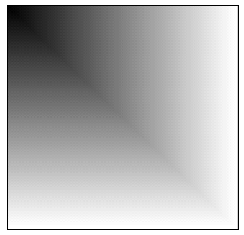
\includegraphics[width=2.9cm]{\networksfigsdir/uniform_attachment_graphon.pdf}
  };
  \end{scope}  
  \begin{scope}[xshift=4.8cm]
    \node [mybox] (box){
    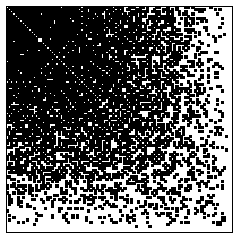
\includegraphics[width=2.8cm]{\networksfigsdir/uniform_attachment_empirical.pdf}
  };
  \end{scope}
\end{tikzpicture}

  \end{center}
 \caption{\emph{Left:} Any exchangeable random graph with vertex set $\Nats$ and edges ${E=(\darray_{ij})_{i,j\in\Nats}}$ can be represented
   by a random function ${\Theta:[0,1]^2\rightarrow[0,1]}$. Given $\AHfunction$, a graph can be sampled by generating a uniform random 
   variable $\AHvar_i$ for each vertex $i$, and sampling edges as ${\darray_{ij}\sim\Bernoulli(\AHfunction(\AHvar_i,\AHvar_j))}$.
   \emph{Middle:} A heat map of an example function $\AHfunction$.
   \emph{Right:} A ${100\times 100}$ symmetric adjacency matrix sampled from $\AHfunction$.
   Only unordered index pairs $\darray_{ij}$ are sampled in the symmetric case. Rows and columns are ordered
   by increasing value of $\AHvar_i$, rather than $i$.}
 \label{fig:W:graph}
\end{figure}


\section{Background: Exchangeable graphs and arrays}
\label{sec:background}

\def\rweightedG{H}
\def\rgraph{G}
\def\SGinf{\mathbb{S}_{\infty}}

A fundamental assumption %\fTBD{Perhaps... or not.  Regardless, this point seems rather unrelated to the task at hand.} 
of Bayesian modeling is that there exists a random variable $\AHfunction$, the parameter of the model, which in some suitable sense decouples the data.
De Finetti's theorem \citep{Kallenberg:2005} 
addresses this problem for random sequences: Let $\darray_1,\darray_2,\ldots$ be a sequence of random variables, each taking values
in a common space $\dataspace$. Recall that the sequence is called \emph{exchangeable} if its joint distribution 
is invariant under arbitrary permutation of the indices, \ie if
\begin{equation}
  \label{eq:exchangeability}
  (\darray_1,\darray_2,\ldots) \eqdist (\darray_{\pi(1)},\darray_{\pi(2)},\ldots) \qquad\text{ for all } \pi\in\SGinf\;.
\end{equation}
Here, $\eqdist$ denotes equality in distribution, and $\SGinf$ is the set of all permutations of $\Nats$ which permute at most a finite number of elements.
De Finetti's theorem states that, $(\darray_i)_{i\in\Nats}$ is exchangeable if and only if there exists a random probability measure $\AHfunction$ on $\dataspace$
such that $\darray_1,\darray_2,\ldots\simiid\AHfunction$. In other words, observations are conditionally \iid given $\AHfunction$. For the purposes of statistics,
this implies that $\AHfunction$ represents common structure in the observed data---the target of statistical inference---whereas $\darray_i|\AHfunction$ represents
remaining, independent randomness in each observation. 



\subsection{De Finetti-type representations for random matrices}

To specify Bayesian models for graph- or array-valued data, we need a suitable counterpart to de Finetti's theorem applicable
when the infinite random sequences in \eqref{eq:exchangeability} are substituted by infinite random arrays $\darray=(\darray_{ij})_{i,j\in\Nats}$.
For such data, the invariance assumption \eqref{eq:exchangeability} is typically too restrictive:
In the graph case $\darray_{ij}\in\lbrace 0,1\rbrace$, for example, the probability of $\darray$ would then depend only on the proportion of present edges
in the graph, but not on the graph structure. Instead, we define exchangeability of random 2-arrays
in terms of the \emph{simultaneous} application of a permutation to rows and columns. More precisely:
\begin{definition}
  An array $\darray=(\darray_{ij})_{i,j\in\Nats}$ is called an \emph{exchangeable array} if 
  \begin{equation}
    \label{eq:jointly:ex}
    (\darray_{ij})\eqdist(\darray_{\pi(i)\pi(j)}) \qquad\text{ for every }\pi\in\SGinf\;.
  \end{equation}
\end{definition}
Since this weakens the hypothesis \eqref{eq:exchangeability} by demanding invariance only under a subset of all permutations of
$\Nats^2$---those of the form $(i,j)\mapsto(\pi(i),\pi(j))$---we can no longer expect de Finetti's theorem to hold.
The relevant generalization of the de Finetti theorem to this case is the following:
\begin{thm}[Aldous, Hoover]
  \label{theorem:ah}
  A random matrix $(\darray_{ij})$ is exchangeable if and only if there is a random (measurable) function ${F:[0,1]^3\rightarrow\dataspace}$ such that the following holds: If $(\AHvar_i)_{i\in\Nats}$ and $(\AHvar_{ij})_{ij\in\Nats}$ are \iid sequences of ~$\Uniform[0,1]$ random variables, then
  \begin{equation}
    \label{eq:ah}
    (\darray_{ij})\eqdist (F(\AHvar_i,\AHvar_j,\AHvar_{ij})) \qquad\text{ for all }i,j\in\Nats\;.
  \end{equation}
\end{thm}


\subsection{Random graphs}

The graph-valued data case $\dataspace=\lbrace{0,1}\rbrace$ is of particular interest. Here, the array $\darray$, interpreted as 
an adjacency matrix, specifies a random simple graph with vertex set $\Nats$. If $\darray$ is symmetric, the graph is undirected. We call a 
random graph exchangeable if $\darray$ satisfies \eqref{eq:jointly:ex}, \ie if its distribution is invariant under permutation of vertices.

For graphs, the representation \eqref{eq:ah} simplifies further:
For any exchangeable random graph, there is a random
function ${\AHfunction:[0,1]^2\rightarrow[0,1]}$ such that
\begin{equation}
  \label{eq:ah:graphon:case}
  %(\darray_{ij})\eqdist 
  F(\AHvar_i,\AHvar_j,\AHvar_{ij}):=\mathbb{I}\lbrace \AHvar_{ij} < \AHfunction(\AHvar_i,\AHvar_j)\rbrace\;.
\end{equation}
Each variable $\AHvar_i$ is associated with a vertex, each variable $\AHvar_{ij}$ with an edge. 
The representation \eqref{eq:ah:graphon:case} is equivalent to the sampling scheme
\begin{equation}
  \label{eq:W:graph}
  \AHvar_1,\AHvar_2,\dots\simiid\Uniform[0,1]\qquad\text{and}\qquad (i,j)\sim\Bernoulli(\AHfunction(\AHvar_i,\AHvar_j))\;,
\end{equation}
which is illustrated in Fig.~\ref{fig:W:graph}. If the graph is undirected, edges are sampled only for unordered index pairs as $\AHvar_{\lbrace ij\rbrace}$,
and it is sufficient to consider symmetric functions $\AHfunction$.

Recent work in discrete analysis shows that any
measurable function $[0,1]^2\rightarrow[0,1]$ can be regarded as a (suitably defined) limit of adjacency matrices
of graphs of increasing size \citep{Lovasz:Szegedy:2006}---intuitively speaking, 
as the number of rows and columns increases, the
matrix in Fig.~\ref{fig:W:graph} (right) converges to the heat map in Fig.~\ref{fig:W:graph} (middle).
The figure also illustrates that convergence, and hence the parametrization of the random graph distribution
by $\AHfunction$, are only unique up to a reordering of rows and columns.

In particular, if we fix an instance ${\AHfunction=\theta_0}$ and generate a random graph according to \eqref{eq:W:graph},
we asymptotically recover the function $\theta_0$. This can be regarded as analogous to the law of large
numbers, guaranteeing that a distribution can asymptotically be recovered from a sample.


\subsection{The general case: $d$-arrays}

Theorem \ref{theorem:ah} can in fact be stated in a more general setting than matrices, namely for random $d$-arrays, which are collections
of random variables of the form $(\darray_{i_1\dots i_d})_{i_1,\dots,i_d\in\Nats}$. Thus, a sequence is a $1$-array, a matrix a $2$-array. A $d$-array 
can be interpreted as an encoding of a relation between $d$-tuples.
In this general case, Theorem \ref{theorem:ah} still holds, but the random function $F$ in \eqref{eq:ah} is in general more complex:
In addition to the collections $\AHvar_{\lbrace i\rbrace}$ and $\AHvar_{\lbrace ij\rbrace}$ of uniform variables, the representation requires an additional
collection $\AHvar_{\lbrace i_j\rbrace_{j\in I}}$ for any non-empty subset $I$ of the set $\lbrace 1,\ldots,d\rbrace$; \eg
$\AHvar_{i_1 i_3 i_4}$ for $d\geq 4$ and ${I=\lbrace 1,3,4\rbrace}$. The representation \eqref{eq:ah} is then substituted by
\begin{equation}
  F:[0,1]^{2^d-1}\longrightarrow\dataspace\qquad\text{and}\qquad \darray_{i_1,\dots,i_d}=F(\AHvar_{I_1},\dots,\AHvar_{I_{(2^d-1)}})\;.
\end{equation}
For $d=1$, we recover de Finetti's theorem. In particular, if $\dataspace=\mathbb{R}$, $F$ is given by the inverse cumulative distribution function
of the random measure guaranteed by de Finetti's theorem.
For a discussion of convergence properties of general arrays similar to those sketched above for random graphs, see 
\citep{Aldous:2009}.

Since we do not explicitly consider the case $d>2$ in our experiments, we restrict 
our presentation throughout to the matrix-valued case for simplicity. We note, however, that the model and inference algorithms described in the
following are applicable to general array-valued data.






\section{Model}

To define a Bayesian model for matrix- or graph-valued data, we start with Theorem \ref{theorem:ah}: A distribution on exchangeable matrices
can be specified by specifying a distribution on measurable functions $[0,1]^3\rightarrow\dataspace$. 
We decompose the function $F$ into two functions 
${\AHfunction:[0,1]^2\rightarrow\latentspace}$ 
and ${H:[0,1]\times\latentspace\rightarrow\dataspace}$ for a suitable space $\latentspace$ , such that
\begin{equation}
  \label{eq:decomposition}
  F(\AHvar_i,\AHvar_j,\AHvar_{ij})=H(\AHvar_{ij},\AHfunction(\AHvar_i,\AHvar_j))\;.
\end{equation}
Such a decomposition always exists---trivially, choose $\latentspace=[0,1]^2$.
Equivalently, there is a conditional probability $P[\,.\,|\AHfunction]$ on $\dataspace$ such that
\begin{equation}
  \label{eq:decomposition:sampling}
  F(\AHvar_i,\AHvar_j,\AHvar_{ij})\sim P[\,.\,|\AHfunction(\AHvar_i,\AHvar_j)]\;.
\end{equation}
Thus, \eqref{eq:decomposition} can be interpreted as a decomposition into a variable $\AHfunction$---the model parameter in terms of Bayesian statistics---which captures the structure of the underlying graph or array,
and random noise represented by $H$ or $P$, respectively.

To define a model, we assume $\AHfunction$ to be continuous, and to be distributed according to a Gaussian process. More precisely,
we set ${\latentspace = \Reals}$ and consider a zero-mean Gaussian process on 
$\cfspace_{\latentspace}:=\cfspace([0,1]^2,\latentspace)$, the space of continuous functions $[0,1]^2\rightarrow\latentspace$,
with kernel function 
${\kernel:[0,1]^2\times[0,1]^2\rightarrow\latentspace}$.
We assume the following generative model:
\begin{equation}
  \label{eq:model}
  \begin{split}
    \AHfunction\; &\sim\; \GP(0,\kernel) \\
    \AHvar_{1},\AHvar_{2},\ldots\; &\simiid\; \Uniform[0,1] \\
    \darray_{ij}\; &\sim\; \likelihood[\,.\,|\AHfunction_{ij}] \;.
  \end{split}
\end{equation}
Additionally, the kernel may depend on parameters, which we denote by $\covhyppar$.

The decomposition of $F$ introduces a natural set of latent variables $W_{ij}:=\AHfunction(\AHvar_i,\AHvar_j)$, conditional on which the
data is explained as $\darray_{ij}\sim\likelihood[\,.\,|\larray_{ij}]$. 
The parameter space of our the model is the infinite-dimensional space $\cfspace_{\latentspace}$. Hence, the model is nonparametric.

The choice of $P$ depends on the type of data considered, and we are here interested in two cases, graphs and 
real-valued matrices.
In either case, the model first generates a latent matrix $W=(W_{ij})$. 
Depending on the type of data, observations are then generated as follows:
\begin{center}
  \begin{tabular}{llll} 
    Observed data & Sample space & $P[\darray_{ij}\in\,.\,|\larray_{ij}]$  \\
    \midrule
    Graph & $\dataspace=\lbrace{0,1}\rbrace$  & $\Bernoulli(\logistic(\larray_{ij}))$
    \vspace{2pt}\\
    Real matrix & $\dataspace=\mathbb{R}$  & $\mbox{Normal}(\larray_{ij},\sigma_\dataspace^2)$\\
  \end{tabular}
\end{center}
where $\logistic$ is the logistic function, and $\sigma_\dataspace^2$ is a noise variance parameter.

The modeling assumptions we impose in addition to exchangeability are thus (i) that the function $\AHfunction$ is continuous---which implies measurability but is a stronger requirement---and (ii) that it is distributed according to a Gaussian process measure on $\cfspace_{\latentspace}$.
Additionally, (iii) the specific choice of $P$ may or may not introduce an additional assumption.
In the case of graphs, the only assumptions are (i) and (ii), 
as any exchangeable graph can be represented by \eqref{eq:ah:graphon:case} or by the equivalent sampling scheme \eqref{eq:W:graph}.
In the case of real-valued matrices, however, the model additionally assumes that the function 
$H$ in \eqref{eq:decomposition} is of the form
\begin{equation}
  H(\AHvar_{ij},\AHfunction(\AHvar_i,\AHvar_j))\eqdist \AHfunction(\AHvar_i,\AHvar_j)+\varepsilon_{ij} \qquad\text{ where }\qquad \varepsilon_{ij}\sim\mbox{Normal}(0,\sigma)\;.
\end{equation}

The Gaussian process prior favors smooth functions, which will in general result in more interpretable latent space embeddings.
Inference in Gaussian processes is a well-understood problem, and the choice of a Gaussian prior allows us to leverage the 
full range of inference methods available for these models.



\begin{rem}[Dense vs. sparse data]
  The methods described here address random matrices that are \emph{dense}, \ie as the size of a finite, observed $n\times n$ matrix increases,
  the number of non-zero entries (or the number of edges in a graph) grows as $O(n^2)$. Although the Aldous-Hoover theorem is sometimes invoked
  for data such as social networks, it should be kept in mind that network data is typically \emph{sparse}, with $O(n)$ non-vanishing entries.
  Density is an immediate consequence of Theorem \ref{theorem:ah}: For graph data, for example, the asymptotic proportion of present edges is
  ${p:=\int\AHfunction(x,y)dxdy}$, and the graph is hence either empty (for $p=0$) or dense (since
  $O(pn^2)=O(n^2)$). Analogous representation theorems for sparse random graphs are to date an open problem in probability.
\end{rem}



\section{Related work}
\label{sec:Related}

Our model has some noteworthy relations to Gaussian process latent variable models (GPLVM), a dimension-reduction technique
\citep[e.g.][]{Lawrence2009}.  GPLVMs can be applied to relational data, which however requires
the assumption that either the rows or the columns of the random matrix are mutually independent \cite{Lawrence2009}. 
In terms of our model, this
corresponds to kernels of the form $\kernel_\AHvar \otimes I$, where $\otimes$ represents the Kronecker matrix product. From this perspective, the application of our model
to bipartite real-valued matrices with $P[\,.\,|\larray_{ij}]=\mbox{Normal}(\larray_{ij},\sigma)$ can be interpreted as 
a form of co-dimensionality reduction.

For graph data, a flexible parametric model is the eigenmodel of \citet{Hoff2007a}. Available nonparametric models include
nonparametric latent class models \cite{Kemp2006}, the mixed membership stochastic blockmodel (MMSB) \citep{Airoldi2008}.
A recent development is the approach of \citet{Yan:Xu:Qi:2011:1}, referred to by the authors as
sparse matrix-variate Gaussian process blockmodel (SMGB). Although not formalized in terms of exchangeability,
this model does not impose an independence assumptions on either rows or columns, in contrast to the GPLVM and other models.
The approach is by construction restricted to kernels of the form $\kernel_\AHvar^1 \otimes \kernel_\AHvar^2$ which prevents 
explicit modeling of symmetric arrays.
Roy and Teh \citep{Roy2009} present a nonparametric Bayesian model of relational data that approximates 
$\AHfunction$ by a piece-wise constant function whose hierarchical structure is a Mondrian process.

Some examples of the various available models can be succinctly summarized as follows:

\begin{table}[h]
  \centering
  \begin{tabular}{lccl} 
%    \toprule
    \multicolumn{4}{c}{Graph data}\\
    \midrule
    %\addlinespace[2pt]
    %\textcolor{red}{Random function model} 
    Random function model & $\AHfunction$ & $\sim$ & $\GP\,(0, \kernel)$\\
    Latent class \cite{Wang1987} & $\larray_{ij}$ & $=$ & $m_{\AHvar_i\AHvar_j}\,\textrm{where} \,\AHvar_i \in \{1,\ldots,K\}$\\
    Nonparametric latent class \cite{Kemp2006} & $\larray_{ij}$ & $=$ & $m_{\AHvar_i\AHvar_j}\,\textrm{where} \,\AHvar_i \in \{1,\ldots,\infty\}$\\
    Latent distance \cite{Hoff2002} & $\larray_{ij}$ & $=$ & $-|\AHvar_i - \AHvar_j|$\\
    Eigenmodel \cite{Hoff2007a} &$\larray_{ij}$ & $=$ & $\AHvar_i'\Lambda \AHvar_j$\\
    MMSB \cite{Airoldi2008} &$\larray_{ij}$ & $=$ & $z_i'\Lambda z_j\,\textrm{where} \,z_i \sim \textrm{Multinomial}(\AHvar_i)$\\
    Nonparametric latent feature \cite{Miller2009} & $\larray_{ij}$ & $=$ & $\AHvar_i'\Lambda \AHvar_j\,\textrm{where} \,\AHvar_i \in \{0,1\}^\infty$\\
    SMGB \cite{Yan:Xu:Qi:2011:1} & $\AHfunction$ & $\dist$ & $\GP\,(0, \kernel_1 \otimes \kernel_2)$ \\
    %\midrule
    \addlinespace[4pt]
    \multicolumn{4}{c}{Real-valued matrix data}\\
    \midrule
    %\textcolor{red}{Random function model} 
    Random function model & $\AHfunction$ & $\sim$ & $\GP\,(0, \kernel)$\\
    Mondrian process~\cite{Roy2009} & $\AHfunction$ & = & piece-wise constant random function\\
    PMF~\cite{Salakhutdinov2008} & $\larray_{ij}$ & $=$ & $\AHvar_i'V_j$\\
    GPLVM~\cite{Lawrence2009} & $\AHfunction$ & $\sim$ & $\GP\,(0, \kernel \otimes I)$\\
    Linear relational GP~\cite{Yu} & $\AHfunction$ & $\sim$ & $\GP\,(0, \kernel_1 \otimes \kernel_2)\,\textrm{where} \,\kernel_i\,\textrm{is linear} $\\
%\bottomrule
\end{tabular}
\label{table:ModelComparison}
\end{table}

The representation \eqref{eq:decomposition:sampling} 
thus provides a common perspective on a range of models in the literature. All models based 
on Gaussian priors and assume $\AHfunction$ to be continuous.
Continuous functions are dense in the space of measurable functions, \ie any measurable function can be arbitrarily well approximated 
by a continuous one. The potentially critical smoothness assumption is therefore not continuity assumption, but rather the 
lengthscale of the Gaussian process.

%% The strategy pursued in the model's definition---start with an exchangeability theorem and define a prior distribution on
%% the representing function---is analogs to more canonical approaches in the de Finetti case, which define priors with
%% large support on the random measure $\AHfunction$ in de Finetti's theorem. Defining a prior that can generate any measurable function
%% $F$ would constitute a ``fully nonparametric'' model, in analogy to early work in Bayesian nonparametrics which attempted to
%% define completely general priors on random measures; 
%% the Dirichlet process was originally conceived with this purpose in mind, but soon turned out to concentrate on the subset of
%% discrete measures \cite{}. To this day, such general priors remain elusive \cite{}.
%% In contrast, nonparametric priors that impose sufficiently strong assumptions to guarantee tractability have proven a very fruitful




\section{Posterior computation}
\label{sec:Inference}

In this section, we describe Markov Chain Monte Carlo (MCMC) algorithms for generating approximate samples from the posterior distribution of the model parameters given a partially observed array.  Most importantly, we describe a random subset-of-regressors approximation that scales to graphs with hundreds of nodes and tens of thousands of edge observations. Given the relatively straightforward nature of the proposed algorithms and approximations, we refer the reader to other papers whenever appropriate.

\subsection{Latent space and kernel}

The random function representation in Theorem \ref{theorem:ah} is not contingent on the use of uniform distributions 
for the variables $\AHvar_i$ and $\AHvar_{ij}$. From a theoretical point of view, any non-atomic
probability measure on a Borel space is valid. For the presentation in Sec.~\ref{sec:background}, 
the domain $[0,1]^2$ of the uniform provides an intuitive analogy
with adjacency matrices. For the purposes of inference, normal distributions are more convenient, and we henceforth use
${\AHvar \dist \Normal(0, I_r)}$ for some integer $r$.

Since we focus on undirected graphical data, we require the symmetry condition $\AHfunction_{ij} = \AHfunction_{ji}$. This can be achieved by constructing the kernel function in the following way
\begin{eqnarray}
\kernel(\inputpoints_1, \inputpoints_2) & = & \frac{1}{2}\big(\bar\kernel(\inputpoints_1, \inputpoints_2) + \bar\kernel(\inputpoints_1, \bar\inputpoints_2)\big) + \sigma^2I \quad \quad \textrm{(Symmetry + noise)} \\
\bar\kernel(\inputpoints_1, \inputpoints_2) & = & \scalefactor^2\exp(-|\inputpoints_1 - \inputpoints_2|^2/(2\lengthscale^2)) \quad \quad \quad \quad \quad \textrm{(RBF kernel)}
\end{eqnarray}
where $\inputpoints_k = (\AHvar_{i_k}, \AHvar_{j_k})$, $\bar\inputpoints_k= (\AHvar_{j_k}, \AHvar_{i_k})$ and $\scalefactor, \lengthscale, \sigma$ represent a scale factor, length scale and noise respectively. This construction can be justified as the limit of a basis function argument with the symmetry condition enforced, analogous to arguments for other kernel functions.
%, but the construction of kernels that preserve certain symmetries is potentially an interesting area for future research.


\subsection{Sampling without approximating the model}

\newcommand{\numobs}{\mathsf o}
\newcommand{\numnodes}{\mathsf n}
In the simpler case of a real-valued array $\darray$, we construct an MCMC algorithm over the variables $(\AHvar,\covhyppar, \sigma_\darray)$ by repeatedly slice sampling \citep{MR1994729} from the conditional distributions
\[
\covhyppar_i \given \covhyppar_{-i}, \sigma_\darray, \AHvar, \darray
\qquad\quad
\sigma_\darray \given \covhyppar, \AHvar, \darray
\qquad\quad \text{and} \qquad\quad
\AHvar_j \given \AHvar_{-j}, \covhyppar, \sigma_\darray, \darray.
\]
Let $\numnodes = |\AHvar_{\lbrace i\rbrace}|$ denote the number of rows in the observed array,
let $\inputpoints$ be the set of all pairs $(\AHvar_i,\AHvar_j)$ for all observed relations $\darray_{ij}$, 
let $\numobs = |\inputpoints|$ denote the number of observed relations,
and 
let $\kernel$ represent the $\numobs \times \numobs$ kernel matrix between all points in $\inputpoints$. Changes to $\covhyppar$ affect every entry in the kernel matrix $K$ and so, naively, the computation of the Gaussian likelihood of $\darray$ takes $\CompOrder(\numobs^3)$ time.  Likewise, changes to $\AHvar$ also affect entries in $K$. Naively reevaluating the Gaussian likelihood term again takes $\CompOrder(\numobs^3)$ time, and so, across all $\numnodes$ rows, we expend $\CompOrder(\numobs^3 \numnodes)$ time. Whether or not this can be improved by exploiting structure in the modifications, the cubic dependence on $\numobs$ seems unavoidable, and thus this naive algorithm is unusable for all but small data sets. 


\subsection{A random subset-of-regressor approximation}

In order to scale the method to much larger graphs, we applied a sparse approximation method known as Subsets-of-Regressors, or simply SoR \citep{Smola01,Wahba99,Silverman1985}. (See \citep{Quinonero-Candela:2005} for an excellent survey of this and other sparse approximations.)  The SoR approximation replaces the infinite dimensional GP with a finite dimensional approximation. Our approach is to treat both the inputs and outputs of the GP as latent variables.
%, a random version of the SoR approximation appears to work very well, even with few pseudoinputs (see below).

In particular, 
introduce $k$ Gaussian distributed pseudoinputs $\pseudopoints=(\pseudopoints_1,\dotsc,\pseudopoints_k)$, and, for each $j=1,\dotsc,k$, define target values ${\targets_j = \AHfunction(\pseudopoints_j)}$.  In other words, writing $K_{\pseudopoints\pseudopoints}$ for the kernel matrix formed from the pseudoinputs $\pseudopoints$, we have
\[
\pseudopoints \dist \Normal(0,I_{2r}) \qquad\text{and}\qquad
\targets \given \pseudopoints \dist \Normal(0,K_{\pseudopoints\pseudopoints}).
\]
The idea of the SoR approximation is to replace $\larray_{ij}$ with the posterior mean conditioned on $(\pseudopoints,\targets)$,
\[
\larray = K_{\inputpoints\pseudopoints} K_{\pseudopoints\pseudopoints}^{-1}\targets,
\label{eqn:GPConditional}
\]
where $K_{\inputpoints\pseudopoints}$ is the kernel matrix between the latent embeddings $\inputpoints$ and the pseudoinputs $\pseudopoints$.  By considering random pseudoinputs, we construct an MCMC variant of the techniques proposed in~\cite{Titsias2008}.
% in be seen to be doing a Bayesian version of sparse variational techniques proposed by Titsias and Lawrence \cite{Titsias2010}.

Given this approximate model, the conditional distribution $\targets \given \AHvar, \pseudopoints, \covhyppar, (\sigma_\darray), \darray$ is amenable to elliptical slice sampling \citep{murray2010}, for both real valued and binary $\darray$. All other random parameters can again be sampled from their full conditional distributions using slice sampling.  The sampling algorithms require that one computes expressions involving~\eqref{eqn:GPConditional}. As a result they cost at most $\CompOrder(k^3 \numobs)$

%These sampling algorithms now require that one recomputes at most $K_{\pseudopoints\pseudopoints}^{-1}$ (or more precisely the Cholesky decomposition) and $K_{\inputpoints\pseudopoints}^{-1}$.  As a result, they cost at most $\Theta(k^3 \numobs)$ time. 

\section{Experiments}

We evaluate the model on three different network data sets. Two of these data sets---the high school and NIPS co-authorship data---have been extensively
analyzed in the literature. The third data set, a protein interactome, was previously noted by \citet{Hoff2007a}
 to exhibit block structure and transitivity.

\begin{center}
  \begin{tabular}{l  l  c  l}
    Data set & Recorded data & Vertices & Reference\\
    \midrule
    High school & high school social network & 90 & e.g.\ \cite{Hoff2007a} \\
    NIPS & densely connected subset of coauthorship network & 234 & e.g.\ \cite{Miller2009} \\
    Protein & protein interactome & 230 & e.g.\ \cite{Hoff2007a}\\
  \end{tabular}
\end{center}

\begin{figure}[]
  \centering
  \begin{tikzpicture}%[transform canvas={xshift=-1cm,yshift=0cm}]
  %\path[use as bounding box] %,fill=white!50!black]
  %  (-4,3) rectangle (14,-3);
  \begin{scope}[xshift=0cm]
    \node [mybox] (box){
      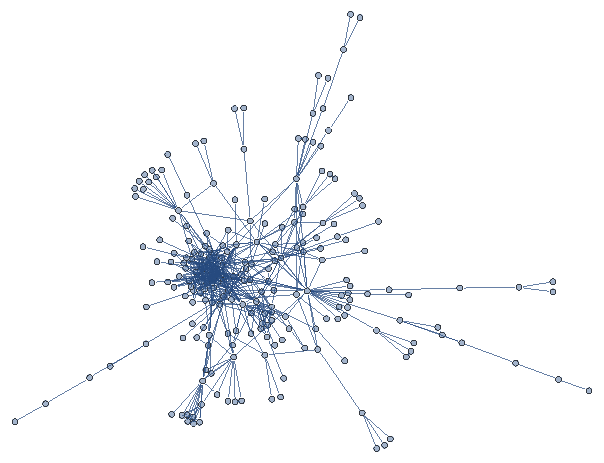
\includegraphics[width=5cm,height=4cm,angle=90]{\networksfigsdir/graph_standard.pdf}
    };
  \end{scope}
  \begin{scope}[xshift=4.5cm]
    \node [mybox] (box){
      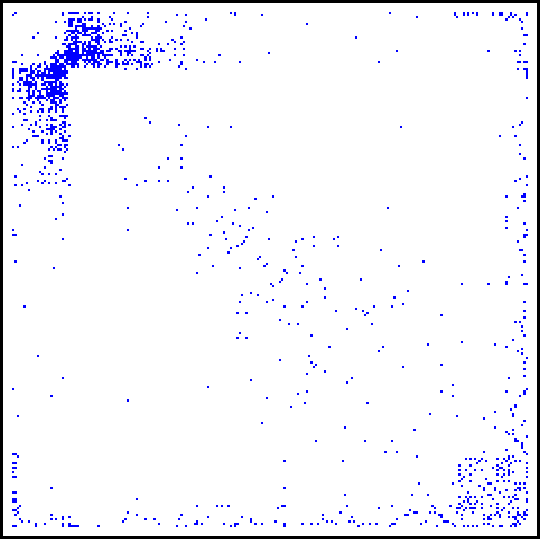
\includegraphics[width=3.5cm]{\networksfigsdir/interactome_adjacency_mathematica.pdf}

  };
  \end{scope}  
  \begin{scope}[xshift=9.2cm]
    \node [mybox] (box){
      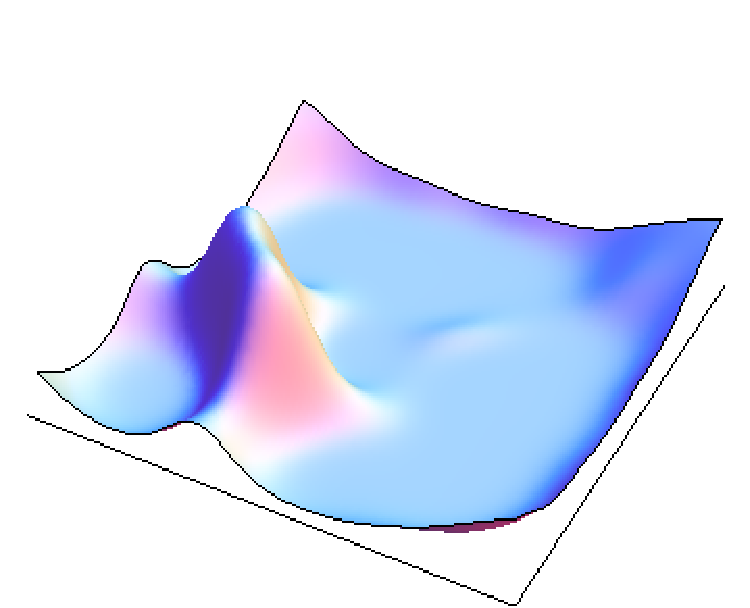
\includegraphics[width=5cm]{\networksfigsdir/graphon_listplot_bmp.pdf}
  };
  \end{scope}
\end{tikzpicture}

  \vspace{-0.5cm}
  \caption{Protein interactome data. 
    \emph{Left:} Interactome network. 
    \emph{Middle:} Sorted adjacency matrix. The network exhibits stochastic equivalence 
    (visible as block structure in the matrix) and homophily (concentration of points around the diagonal). 
    \emph{Right:} Maximum a posteriori estimate of the function $\AHfunction$, corresponding to the function in Fig.~\ref{fig:W:graph} (middle).
  }
  \label{fig:(R)GPLVM_Comparison}
\end{figure}


We compare performance of our model on these data sets to three other models, probabilistic matrix factorization (PMF) \cite{Salakhutdinov2008},
Hoff's eigenmodel, which models the adjacency matrix using a low-rank approximation, followed by a sigmoid transformation, and the GPLVM (see also Sec.~\ref{sec:Related}). The models are chosen for comparability, since they all embed nodes into a Euclidean latent space.
%All of these models represent nodes as being embedded in a latent space, although the approaches vary considerably.
Experiments for all three models were performed using reference implementations by the respective 
authors.\footnotemark

\footnotetext{Implementations are available for PMF at
http://www.mit.edu/\texttildelow rsalakhu/software.html;
for the eignmodel at
http://cran.r-project.org/src/contrib/Descriptions/eigenmodel.html;
and for the GPLVM at
http://www.cs.man.ac.uk/\texttildelow neill/collab/ .}

\begin{center}
  \begin{tabular}{l  l  c  l }
    Model & Method & Iterations [burn-in] & Algorithm parameters\\
    \midrule
    PMF \cite{Salakhutdinov2008} & stochastic gradient & 1000 & author defaults
    \\
    Eigenmodel \cite{Hoff2007a} & MCMC & 10000 [250] & author defaults
    \\
    GPLVM \cite{Lawrence2009} & stochastic gradient  & 20 sweeps & author defaults
    \\
    Random function model & MCMC & 1000 [200] & (see below)
  \end{tabular}
  %\label{table:DataSets}
  %\end{table}
\end{center}


Common practice for many latent variable models relying on MCMC is to inatialise the sampler using 
result from another model to reduce mixing time. Experiments show that results for our inference algorithm
do not depend strongly on the choice of initialization method, provided that the initialization is reasonable.
The results reported here are initialized using a GPLVM embedding.
We use standard normal 
priors on the latent variables $\AHvar$ and $\AHvaralt$, and log normal priors for kernel parameters.
\vspace{-0.32cm}
\parpic(6cm,2.7cm)[r]{
\begin{minipage}[h]{8cm}
\begin{center}
  \begin{tabular}{c | c c c}
    {} & log mean & std & width \\
    \midrule
    length scale & 1 & 0.5 & 0.5 \\
    scale factor & 2 & 0.5 & 0.5 \\
    target noise & 0.1 & 0.5 & 0.1 \\
    $\AHvar$ & - & - & 4 \\
    $\pseudopoints$ & - & - & 2
  \end{tabular}
\end{center}
\end{minipage}}
Slice sampling parameters are chosen to favor slice sampling acceptance after a reasonable number of iterations, as evaluated over
a range of data sets. Specific values of prior and sampling parameters are summarized in the table on the right.

In all experiments, we partitioned the edge data into 5 equally sized partitions and performed 5-fold cross validation, predicting the links in one held out partition given the other 4. 
Where the models did not restrict their outputs to values between 0 and 1, we truncated any predictions lying outside this range.
The following table reports average AUC (area under ROC) for the various models, with numbers for the top performing model set in bold.
Significance of results is evaluated by means of a $t$-test with a $p$-value of 0.05; results for models not distinguishable from the top performing model
in terms of this $t$-test are also set in bold. \fPROBLEM{The erroneous 0.494 (PMF, NIPS 3) should actually be 0.820}

\begin{center}
  \begin{tabular}{r | r r r | r r r | r r r}
    \multicolumn{10}{c}{AUC results} \\
    \addlinespace[2pt]
    Data set & \multicolumn{3}{c|}{High school} & \multicolumn{3}{c|}{NIPS} & \multicolumn{3}{c}{Protein} \\
    Latent dimensions & 1 & 2 & 3 & 1 & 2 & 3 & 1 & 2 & 3 \\
    \midrule
    PMF                   & 0.747 & 0.792 & 0.792 & 0.729 & 0.789 & 0.494 & 0.787 & 0.810 & 0.841 \\
    Eigenmodel            & 0.742 & \textbf{0.806} & \textbf{0.806} & 0.789 & 0.818 & 0.845 & 0.805 & 0.866 & 0.882 \\
    GPLVM                 & 0.744 & 0.775 & 0.782 & \textbf{0.888} & 0.876 & 0.883 & 0.877 & \textbf{0.883} & 0.873 \\
    RFM & \textbf{0.780} & \textbf{0.813} & 0.654 & \textbf{0.902} & \textbf{0.930} & \textbf{0.926} & \textbf{0.898} & \textbf{0.891} & \textbf{0.901} \\
  \end{tabular}
\end{center}

The random function model outperforms the other models in almost all tests. We also note that in most experiments, a single latent dimension
suffices to achieve better performance, even when the other models use additional latent dimensions.

The posterior distribution of $\AHfunction$ favors functions defining random array distributions which explain the data well. In this sense,
our model fits a probability distribution. The standard inference methods for GPLVM and PMF applied to relational data, in contrast, are designed to fit mean squared error, and should therefore
be expected to show stronger performance under a mean squared error metric. As the following table shows, this is indeed the case.
The reported values are RMSE results,  with significance evaluated as above.

\begin{center}
  \begin{tabular}{r | r r r | r r r | r r r}
    \multicolumn{10}{c}{RMSE results} \\
    \addlinespace[2pt]
    Data set & \multicolumn{3}{c|}{High school} & \multicolumn{3}{c|}{NIPS} & \multicolumn{3}{c}{Protein} \\
    Latent dimensions & 1 & 2 & 3 & 1 & 2 & 3 & 1 & 2 & 3 \\
    \midrule
    PMF                   & 0.245 & 0.242 & 0.240 & 0.141 & 0.135 & 0.130 & 0.151 & 0.142 & 0.139 \\
    Eigenmodel            & 0.244 & \textbf{0.238} & \textbf{0.236} & 0.141 & 0.132 & 0.124 & 0.149 & 0.142 & \textbf{0.138} \\
    GPLVM                 &0.244 & 0.241 & 0.239 & \textbf{0.112} & \textbf{0.109} & \textbf{0.106} & \textbf{0.139} & \textbf{0.137} & \textbf{0.138} \\
    RFM & \textbf{0.241} & \textbf{0.236} & 0.248 & 0.126 & \textbf{0.115} & \textbf{0.109} & 0.144 & 0.141 & 0.140 \\
  \end{tabular}
\end{center}

An arguably more suitable metric is comparison in terms of log-likelihoods. These cannot, however, be computed in a meaningful manner for
models such as PMF and GPLVM, which assign a Gaussian likelihood to data. The next table hence reports only comparisons to the eigenmodel.
%This table is negative conditional log likelihood * 1000 / (number of predicted links).
\begin{center}
  \begin{tabular}{r | r r r | r r r | r r r}
     \multicolumn{10}{c}{Negative conditional log-likelihood} \\
     \addlinespace[2pt]
     Data set & \multicolumn{3}{c|}{High school} & \multicolumn{3}{c|}{NIPS} & \multicolumn{3}{c}{Protein} \\
    Latent dimensions & 1 & 2 & 3 & 1 & 2 & 3 & 1 & 2 & 3 \\
    \midrule
    Eigenmodel & 220 & \textbf{210} & \textbf{200} & 88 & 81 & 75 & 96 & 92 & 86 \\
    RFM        & \textbf{210} & \textbf{200} & 240 & \textbf{71} & \textbf{58} & \textbf{55} & \textbf{83} & \textbf{81} & \textbf{79}  \\
  \end{tabular}
\end{center}

%\textcolor{red}{Wrap-up sentence here.}


\section{Discussion and conclusions}

%% There has been a tremendous amount of research into modelling matrices, arrays, graphs and relational data, but nonparametric
%% Bayesian modeling of such data is essentially uncharted territory. 
%% On the conceptual side, progress has been hamstrung by an apparent lack of mathematical structure,
%% but recent advances in discrete analysis establish an 
%% analytical structure on spaces of graphs and of related objects \citep[e.g.][]{Lovasz:Szegedy:2006}. In principle, the 
%% mathematical tools for the derivation of rigorous statistical results are therefore  in place. Recent work of
%% \citet{Bickel:Chen:Levina:2011} provides an example.

%% In analogy to de Finetti's theorem, the representation results 
%% \citep{Aldous:1981,Hoover:1979,Kallenberg:1992} 
%% precisely map out the scope of possible Bayesian models for exchangeable arrays:
%% Any such model can be interpreted as a prior on random measurable functions on a suitable space.
%% There is so far no systematic understanding of such priors,
%% and how properties of a prior emphasize or discourage specific properties of graphs. 
%% %Considering the popularity of Bayesian methods and 
%% %the growing importance of graph and relational data, there can be little doubt that this is bound to change.
%% To speculate, a clear distinction will probably emerge between models which assume the underlying random function to be
%% discontinuous (such as the Mondrian process \cite{Roy2009})
%% and continuous models, such as our model and most of the models surveyed in Sec.~\ref{sec:Related}.
%% The Gaussian process prior proposed here




There has been a tremendous amount of research into modelling matrices, arrays, graphs and relational data, but nonparametric
Bayesian modeling of such data is essentially uncharted territory. 
In most modelling circumstances, the assumption of exchangeability amongst data objects is natural and fundamental to the model.
In this case, the representation results 
\citep{Aldous:1981,Hoover:1979,Kallenberg:1992} 
precisely map out the scope of possible Bayesian models for exchangeable arrays:
Any such model can be interpreted as a prior on random measurable functions on a suitable space.

Nonparametric Bayesian statistics provides a number of possible priors on random functions, but the Gaussian process
and its modifications are the only well-studied model for almost surely continuous functions.
For this choice of prior, our work provides a general and simple modeling approach that can be motivated directly by the
relevant representation results.
%Inference is then possible using an efficient MCMC algorithm for this model. 
The model results in both interpretable representations for networks, such as a visualisation of a protein interactome, and has 
competitive predictive performance on benchmark data.




%% There has been a tremendous amount of research into modelling matrices, arrays, graphs and relational data. 
%% In most modelling circumstances, the assumption of exchangeability amongst data objects is natural and fundamental to the model.
%% One of the contributions of this paper is to highlight fundamental results in probability theory that justify the use of latent variable models for exchangeable arrays, especially when one employs a nonparametric prior over the functions mapping from latent variables to data. We have also related our work to many other models for graphs and matrices.

%% In this paper we have used a Gaussian process prior to model random functions and have developed an efficient MCMC algorithm for this model. In doing so we have created an MCMC variant of a widely used sparse approximation for Gaussian processes.
%% Our model results in both interpretable representations for networks, such as a visualisation of a protein interactome, and has competitive predictive performance on three benchmark data sets.

\outbpdocument{
\bibliographystyle{plainnat}
\bibliography{references.bib}
}
